\subsection{Stance And Walking Transition}
\subsubsection{Dynamic Model}
the reduced model
linear bipedal model
suppose when standing, we hight vaiation is almost zero.
We only conside the horizontal movement


basicall the stance are divided into three phase

1 Single Support Phase

\begin{equation}
\ddot{y}=t/ml+gy/L
\end{equation}
2 double stance Phase
\begin{equation}
\ddot{y}=(TL+TR)/ML+g/l*wL(y-y_m)+g/l*wr(ym-yr)
\end{equation}
3 fall 
if $ym >d$
than the stance will fall.
The goal of control is confine the flow withing the safe region
\begin{figure}[ht]
  \centering
  \includegraphics[width=3in]{images/uncontrolled.eps}
  \caption{Stance Dynamics}
\end{figure}

\subsubsection{Global And Local Motor Control}
he original system is simmilar to mass spring system.
It wil vibrate continutelly.
\begin{figure}[ht]
  \centering
  \includegraphics[width=3in]{images/AttractiveCircle.eps}
  \caption{Stance Dynamics}
\end{figure}
while in our method ,by coubling neural system the the oscillator, it form a limit circle

But because of the special characteristics of the stancing model, when move out the safe region, 
It will fall.

2 lie group control
By the speed transformation,
The speed we can control the stance motion to move within the safe region.

\begin{figure}[ht]
  \centering
  \includegraphics[width=3in]{images/LieAttractiveCircle.eps}
  \caption{Stance Dynamics}
\end{figure}
then the stance posture is controlled

by the energy transformation,
we can control the final vibration magnitude.
\subsection{Walking Stance Transition}
Application 
Walking and Stance Transformation



\subsubsection{Walk Stance Transition}

walk to stance transform
\begin{figure}[ht]
  \centering
  \includegraphics[width=3in]{images/stanceState.eps}
  \caption{Stance Dynamics}
\end{figure}

when transform from walk to stance, there is no heel impact.
The swing leg touch the ground, it will generate force and start to bend
x only depend on the stance leg
there is a transform f, that transform the state from q to x.
\[
x=f(q).
\]
stance to walk.

Stance to walk happens , the font leg is kept strait, the back leg is becoming strait and rotate.


Walk to Stance Transform

the walk state


From Stance 2 Walk

the black one is on the limit cirle, while the red one is walking start point.

\begin{figure}[ht]
  \centering
  \includegraphics[width=3in]{images/s2walk.eps}
  \caption{Stance Dynamics}
\end{figure}